

\section{Testy}
\subsection{Opisy przeprowadzonych eksperymentów}

Dane testowe składają się ze zbioru prac naukowych pobranych ze stron Arxiv i PMC. Każdy dokument posiada przypisane mu tagi i ilość cytowań w innych pracach naukowych. 



\subsection{Jakość wyszukiwania}

Każdemu dokumentowi została przypisana jego 'jakość'. Jakość dokumentu została określona jako znormalizowana ilości cytowań danego dokumentu w innych pracach naukowych. Należy tutaj zaznaczyć, że przy dodawaniu danych testowych do bazy danych, liczba użytkowników, którzy dodali dany dokument, jest równa ilości cytowań. Może to mieć wpływ na wyniki testów. Jednakże przy obydwu algorytmach, wpływ maja nie tylko użytkownicy, ale również tagi i ich jakość. Dodatkowo, przy tworzeniu macierzy, liczba ta nie jest używana bezpośrednio.



\begin{figure}[tb]
    \centering
    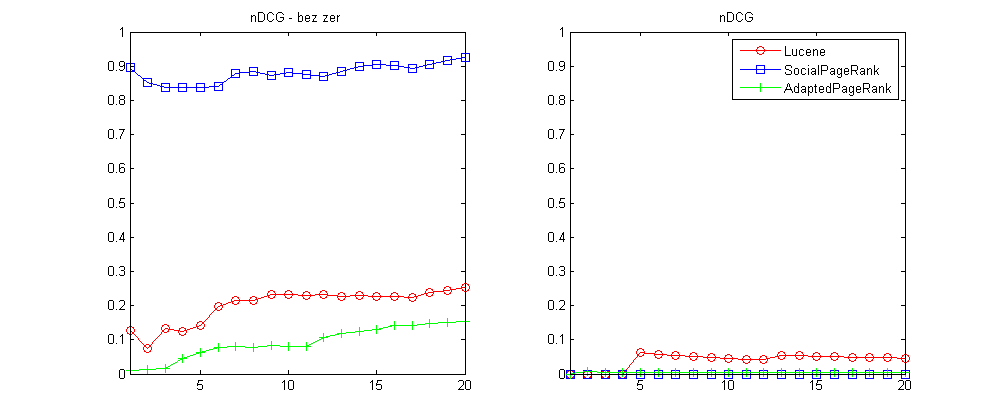
\includegraphics[width=\linewidth]{test_jakosc_genome.png}
    \caption{Wyniki testów pod względem jakości, wyszukiwanie słowa: 'genome'}
    \label{fig:jakosc-genome}

\end{figure}

\begin{figure}[tb]
    \centering
    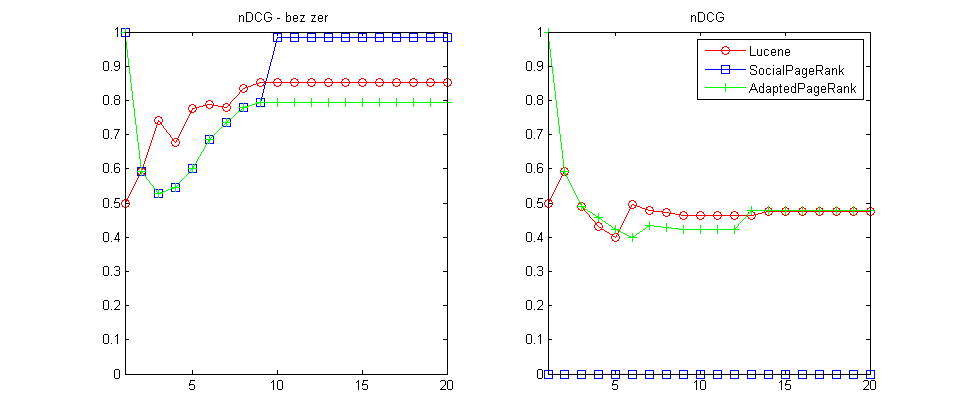
\includegraphics[width=\linewidth]{test_jakosc_hashimoto.png}
    \caption{Wyniki testów pod względem jakości, wyszukiwanie słowa: 'hashimoto'}
    \label{fig:jakosc-hashimoto}

\end{figure}

\begin{figure}[tb]
    \centering
    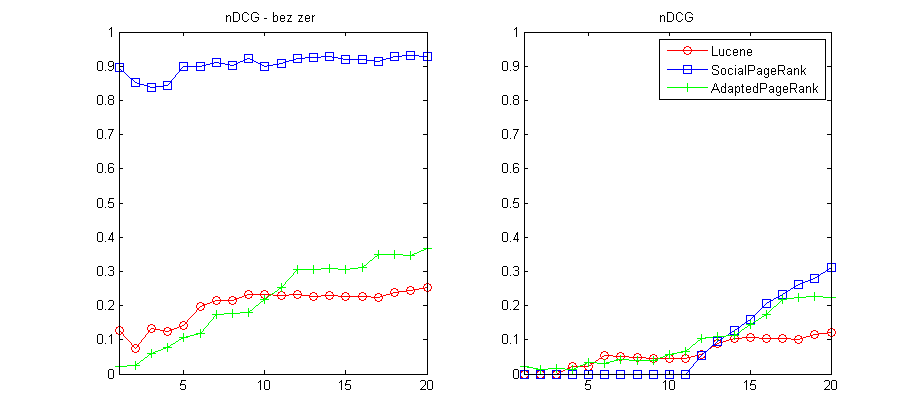
\includegraphics[width=\linewidth]{test_jakosc_immunodeficiency.png}
    \caption{Wyniki testów pod względem jakości, wyszukiwanie słowa: 'immunodeficiency'}
    \label{fig:jakosc-immunodeficiency}

\end{figure}

\begin{figure}[tb]
    \centering
    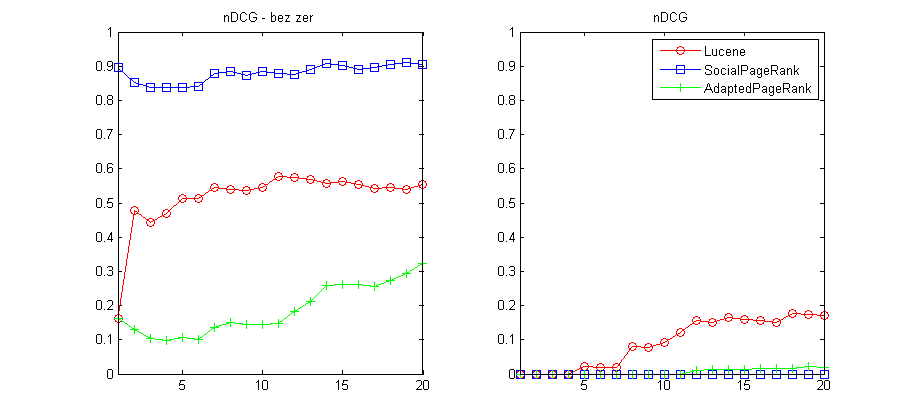
\includegraphics[width=\linewidth]{test_jakosc_pathogen.png}
    \caption{Wyniki testów pod względem jakości, wyszukiwanie słowa: 'pathogen'}
    \label{fig:jakosc-pathogen}

\end{figure}

\begin{figure}[tb]
    \centering
    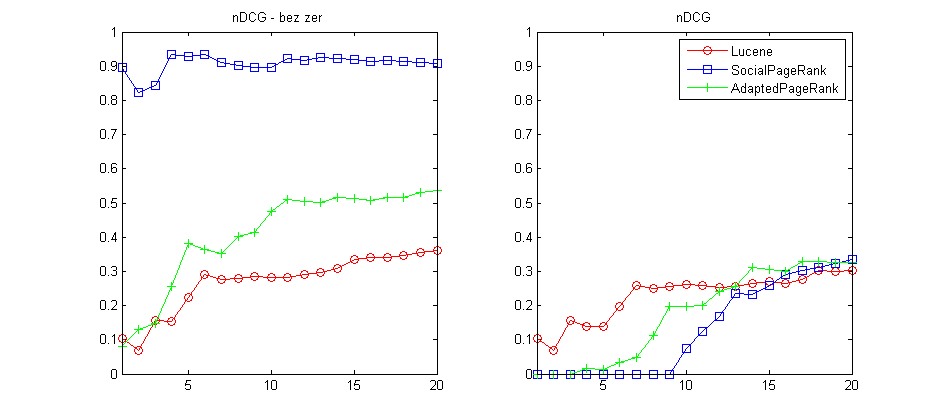
\includegraphics[width=\linewidth]{test_jakosc_retrovirus.png}
    \caption{Wyniki testów pod względem jakości, wyszukiwanie słowa: 'retrovirus'}
    \label{fig:jakosc-retrovirus}

\end{figure}


Miarą testów jest znormalizowany zysk całościowy (ang. Normalized Discounted Cumulative Gain). Wyliczany jest on według wzoru:

\begin{equation}
   nDCG_{p} = \frac{DCG_{p}}{IDCG_{p}} 
\end{equation}

Gdzie DCG to zysk całościowy (ang. Discounted Cumulative Gain), a IDCG to idealny zysk całościowy obliczony jako maksymalny możliwy wynik dla danego zapytania $p$ .

Zysk całościowy wyliczany jest za pomocą wzoru:

\begin{equation}
    DCG_{p} = rel_{1} + \sum_{i=2}^{p} \frac{rel_{i}}{\log_{2}(i+1)} 
\end{equation}

Gdzie $rel_i$ jest jakością dokumentu otrzymanego w wyniku na pozycji $i$.

Testy zostały przeprowadzone na zbiorze wszystkich zebranych dokumentów. Do wyników brane były tylko dokumenty ze zbioru prac naukowych. W przypadku uzyskania w wyniku dokumentu z poza tego zbioru, jakość tego wyniku równa jest zero. Dla porównania przedstawiono również wyniki testów, w których pominięto wyniki z poza zbioru.

Można zauważyć na wykresach, że otrzymujemy lepsze wyniki przy użyciu algorytmu SocialPageRank w zbiorze danych z których usunięto elementy zerowe. Dokumenty otrzymane przy pomocy innych metod są gorszej jakości. 

W zbiorze w którym występowały dokumenty o jakości zero, Lucene i AdaptedPageRank dawały zdecydowanie lepsze wyniki. Mimo, że koszt całościowy jest niski, to w przypadku algorytmu SocialPageRank jest on w większości zerowy. Nawet jeśli jakość tych wyników jest niska, AdaptedPageRank i Lucene dają poprawne wyniki w pierwszych 10 elementach.

Zaobserwować również wysokie wyniki otrzymane przy pomocy Lucene. W tym przypadku, może to byś spowodowane wysoką jakością publikacji naukowych w porównaniu do treści stron internetowych.





\subsection{Precyzja wyszukiwania}



\begin{figure}[tb]
    \centering
    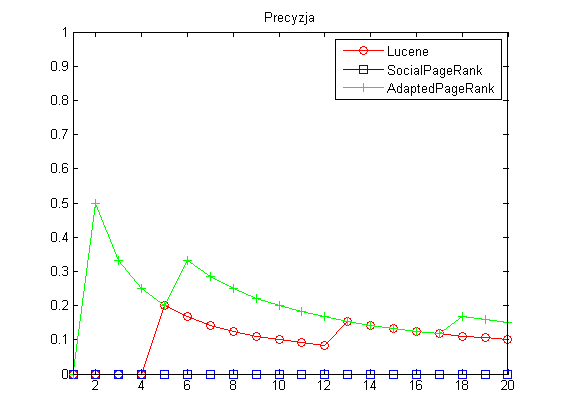
\includegraphics[width=0.9\linewidth]{test_wyniki_prec_genome.png}
    \caption{Wyniki precyzji wyników, wyszukiwanie słowa: 'Genome', }
    \label{fig:prec-genome}

\end{figure}



\begin{figure}[tb]
    \centering
    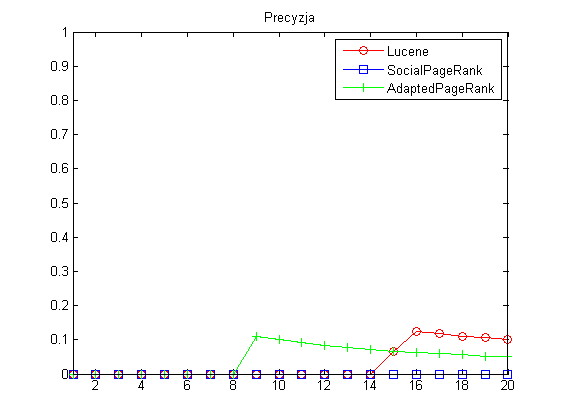
\includegraphics[width=0.9\linewidth]{test_wyniki_prec_geophisics.png}
    \caption{Wyniki precyzji wyników, wyszukiwanie słowa: 'Geophisics', }
    \label{fig:prec-geophisics}

\end{figure}

\begin{figure}[tb]
    \centering
    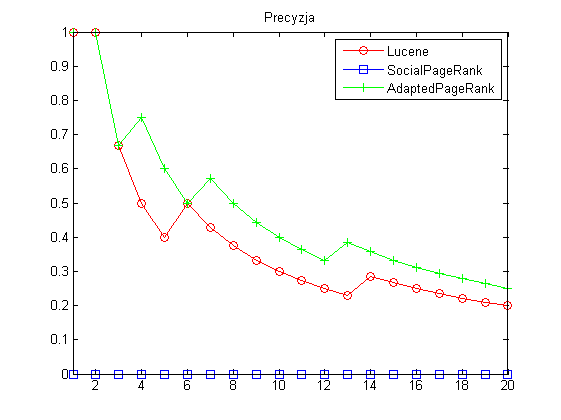
\includegraphics[width=0.9\linewidth]{test_wyniki_prec_hashimoto.png}
    \caption{Wyniki precyzji wyników, wyszukiwanie słowa: 'Hashimoto', }
    \label{fig:prec-hashimoto}

\end{figure}


\begin{figure}[tb]
    \centering
    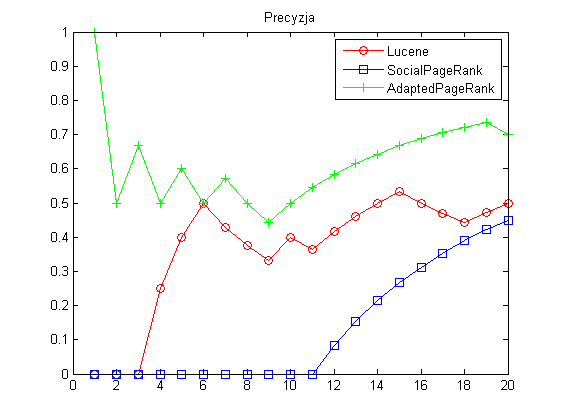
\includegraphics[width=0.9\linewidth]{test_wyniki_prec_immunodeficiency.png}
    \caption{Wyniki precyzji wyników, wyszukiwanie słowa: 'Immunodeficiency', }
    \label{fig:prec-immunodeficiency}

\end{figure}


\begin{figure}[tb]
    \centering
    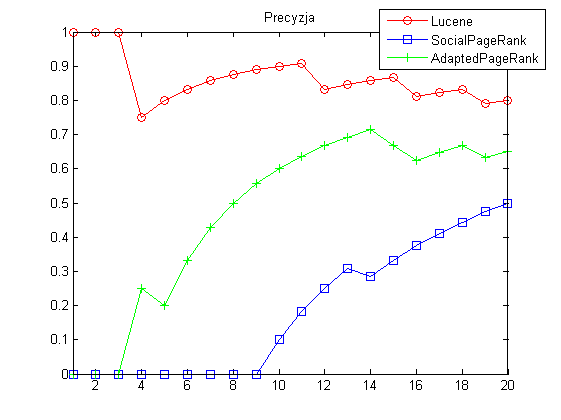
\includegraphics[width=0.9\linewidth]{test_wyniki_prec_retrovirus.png}
    \caption{Wyniki precyzji wyników, wyszukiwanie słowa: 'Retrovirus', }
    \label{fig:prec-retrovirus}

\end{figure}



Kolejną miarą wyników algorytmów jest precyzja. Miara ta będzie sprawdzana dla pierwszych  $n$ wyników:

\begin{equation}
Prec(n) = \frac{number\_rel_n}{n}
\end{equation}

Precyzja dla $n$ jest to ilość poprawnie wybranych elementów ($number\_rel$) dla pierwszych $n$ elementów.


Dla posiadanych danych, precyzja odpowiedzi została przetestowana dla pierwszych 20 wyników. Przykładowe wyniki znajdują się na wykresach \ref{fig:prec-genome},  \ref{fig:prec-geophisics},  \ref{fig:prec-hashimoto},  \ref{fig:prec-immunodeficiency} i  \ref{fig:prec-retrovirus}.



Można zaobserwować, że poza wykresem \ref{fig:prec-retrovirus} i \ref{fig:prec-geophisics} (od elementu 15) najlepsze wyniki uzyskujemy używając algorytmu Adapted PageRank. Przy użyciu Lucene otrzymujemy gorsze wyniki, ale ciągle dość wysokie. Algorytm SocialPageRank w pierwszych 20 wynikach podaje bardzo złe wyniki, często zerowe.



\subsection{Średni wzajemny ranking}


Przeprowadzone zostały również testy biorące pod uwagę cały zbiór
dokumentów, czyli dokumenty zebrane z serwisu delicious.com i dokumenty złożone
z publikacji naukowych. Problemem w testowaniu algorytmów wyszukiwania na
takim dużym zbiorze jest sam proces ocenienia otrzymanych odpowiedzi.  Dodatkowo
należy sprawdzić czy w zbiorze pominiętych dokumentów nie znajdują się
wyniki, które mogą nas interesować. Dlatego też do przeprowadzenia
tych testów użyto miary 'średniego wzajemnego rankingu', która bierze
pod uwagę tylko wybrany zbiór zapytań i jedną szukaną odpowiedz.


Średni wzajemny ranking (MMR, Mean reciprocal rank) jest miarą pozwalającą
na ocenianie jakości wyników zwracanych jako lista elementów
posortowanych według trafności. Kryterium to bierze pod uwagę zbiór
zapytań i jedna poprawna odpowiedz. Mierzona jest pozycja, na której
znajduję się interesująca nas odpowiedz. Dla przykładu, jeśli w
zbiorze zapytań znajduję się fraza 'bbc' oczekujemy, że główna strona
internetowa serwisu informacyjnego BBC będzie na wysokiej pozycji w
rankingu. Im dalej w wynikach znajduje się oczekiwana odpowiedz, tym
gorszy będzie wynik MMR.

Średni wzajemny ranking (MMR) wyrażany jest wzorem:

\begin{equation}
    \text{MRR} = \frac{1}{|Q|} \sum_{i=1}^{|Q|} \frac{1}{\text{rank}_i}
\end{equation}
Gdzie:
\begin{itemize}
\item $Q$ - zbiór zapytań,
\item $rank_i$ - pozycja poprawnego wyniku.
\end{itemize}


Do testów wybrane zostało wybrane dziesięć stron internetowych i zapytania
opisujące je w jednoznaczny sposób. Ponieważ nie zawsze główne strony znajdują się w bazie danych, jako wynik wystarczający uznawana jest również strona będącą w tej samej domenie. Dla przykładu, dla zapytania 'BBC' akceptowane są strony bbc.co.uk i bbc.co.uk/tv jako poprawne odpowiedzi.

 W tabeli \ref{tab:mmr} znajduje się zbiór zapytań i numer pozycji w wynikach, na której otrzymaliśmy poszukiwaną stronę. Wynik zero oznacza brak oczekiwanego wyniku w pierwszych dwudziestu odpowiedziach.

\begin{table}[htb]
  \centering
    \begin{tabular}{ | l | l | l | l | l | }
\hline
  Zapytanie  & Lucene & SocialPageRank & AdaptedPageRank & Inne serwisy \\
\hline
Debian & 7  &  4  & 0  & 0\\
BBC &   2 &  0  & 2  &  5 \\
Intel & 1  & 8  & 0  & 0 \\
Deviantart & 1  & 2  & 0 &  6\\
Pastebin & 1 &  0  & 8 &  3\\
Wikipedia & 4 &  1  & 1 &  14\\
Guardian & 2 &  4  & 1 &  6\\
Youtube & 0  & 0  & 2  & 11 \\
Sourceforge & 3 & 3  & 3 &  2 \\
\hline
\end{tabular}
  \caption{ Pozycja odpowiedzi w wynikach w zależności od algorytmu i zapytania}
  \label{tab:mmr}
\end{table}



Wyniki zostały również przedstawione w postaci figury \ref{fig:wyniki-mmr}. Tak samo jak w pojedynczych winkach jak uśrednionych można zaobserwować, że najlepsze wyniki otrzymujemy przy użyciu frameworku Lucene, czyli algorytmu TF-IDF. 



\begin{figure}[h]
    \centering
    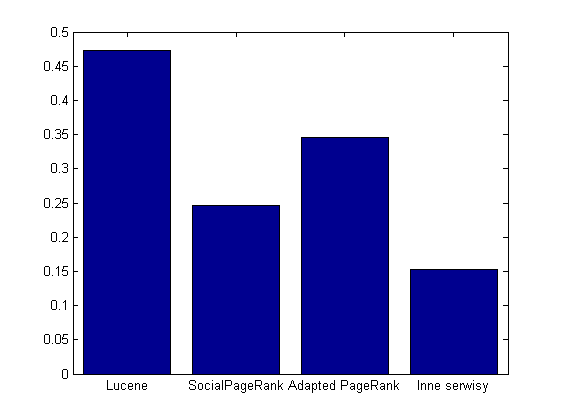
\includegraphics[width=0.9\linewidth]{mmr.png}
    \caption{Średni wzajemny ranking }
    \label{fig:wyniki-mmr}

\end{figure}















